%%%%%%%%%%%%%%%%%%%%%%%%%%%%%%%%%%%%%%%%%%%%%%%%%%%%%%%%%%%%%%%%%%%%%%%%%%%%%%%%
%2345678901234567890123456789012345678901234567890123456789012345678901234567890
%        1         2         3         4         5         6         7         8

%\documentclass[letterpaper, 10 pt, conference]{ieeeconf}  % Comment this line out if you need a4paper
\documentclass[letterpaper, 12 pt, onecolumn, journal]{IEEEtran}  % Comment this line out if you need a4paper

%\documentclass[a4paper, 10pt, conference]{ieeeconf}      % Use this line for a4 paper

\IEEEoverridecommandlockouts                              % This command is only needed if 
                                                          % you want to use the \thanks command

%\overrideIEEEmargins                                      % Needed to meet printer requirements.

% See the \addtolength command later in the file to balance the column lengths
% on the last page of the document

% The following packages can be found on http:\\www.ctan.org
%\usepackage{graphics} % for pdf, bitmapped graphics files
%\usepackage{epsfig} % for postscript graphics files
%\usepackage{mathptmx} % assumes new font selection scheme installed

%\usepackage{amsmath} % assumes amsmath package installed
%\usepackage{amssymb}  % assumes amsmath package installed

\usepackage{color}
\usepackage{listings}
\usepackage{tcolorbox}
\usepackage{amsmath}
\usepackage{amssymb}
\usepackage{algorithm}
\usepackage{graphicx}
\usepackage[noend]{algpseudocode}
\usepackage{times}
\usepackage{url}
\usepackage{tikz}
\usepackage{tcolorbox}
\usepackage{xspace}
\usepackage{drum}
\usepackage{subcaption}
%\usepackage[normalem]{ulem}
%\usepackage{enumitem}
\usepackage{enumerate}
\usepackage{verbatim}

%\captionsetup[subfigure]{labelformat=simple}
%\renewcommand\thesubfigure{(\alph{subfigure})}

\newcommand{\Weazelball}{\textsc{Weazelball}\xspace }
\newcommand{\Wb}{\textsc{Wb}\xspace }
\newcommand{\Gazebo}{\textsc{Gazebo}\xspace }
\newcommand{\CAD}{\textsc{CAD}\xspace }
\newcommand{\Solidworks}{\textsc{Solidworks}\xspace }
\newcommand{\Vicon}{\textsc{Vicon}\xspace }
\newcommand{\Tracker}{\textsc{Tracker}\xspace }
\newcommand{\VRPN}{\textsc{VRPN}\xspace }
\newcommand{\HD}{\textsc{HD}\xspace }
\newcommand{\LED}{\textsc{LED}\xspace }
\newcommand{\IR}{\textsc{IR}\xspace }
\newcommand{\IMU}{\textsc{IMU}\xspace }
\newcommand{\SLERP}{\textsc{SLERP}\xspace }
\newcommand{\FOV}{\textsc{FOV}\xspace}
\newcommand{\DOF}{\textsc{DOF}\xspace}
\newcommand{\ODE}{\textsc{ODE}\xspace}
\newcommand{\markalign}{A}
\newcommand{\marksignal}{B}
\newcommand{\markled}{l}
\newcommand{\melt}{\textbf{\texttt{melt}}\xspace}
\newcommand{\vlc}{\textbf{\texttt{vlc}}\xspace}
\newcommand{\vsk}{\textbf{vsk}\xspace}
\newcommand{\repo}{\textbf{github.com/PositronicsLab/wild-body}}

\definecolor{codegreen}{rgb}{0,0.6,0}
\definecolor{codegray}{rgb}{0.5,0.5,0.5}
\definecolor{codepurple}{rgb}{0.58,0,0.82}
\definecolor{backcolour}{rgb}{0.95,0.95,0.92}
 
\lstdefinestyle{mystyle}{
    backgroundcolor=\color{backcolour},   
    commentstyle=\color{codegreen},
    keywordstyle=\color{magenta},
    numberstyle=\tiny\color{codegray},
    stringstyle=\color{codepurple},
    basicstyle=\footnotesize,
    breakatwhitespace=false,         
    breaklines=true,                 
    captionpos=b,                    
    keepspaces=true,                 
    numbers=left,                    
    numbersep=5pt,                  
    showspaces=false,                
    showstringspaces=false,
    showtabs=false,                  
    tabsize=2
}
 
\lstset{style=mystyle}
\title{\LARGE \bf An Introduction to Automatic Differentiation in Eigen}

\author{Evan Drumwright$^*$% <-this % stops a space
\thanks{$^*$ Toyota Research Institute, Palo Alto, CA, USA}
}

\begin{document}
\maketitle
\thispagestyle{empty}
\pagestyle{empty}

\urlstyle{tt}

%%%%%%%%%%%%%%%%%%%%%%%%%%%%%%%%%%%%%%%%%%%%%%%%%%%%%%%%%%%%%%%%%%%%%%%%%%%%%%%%
\begin{abstract}
Automatic differentiation is a convenient way to compute derivatives that differs from \emph{analytical differentiation}---which uses a human (or computer) to determine derivatives offline and then turn that output into programming code---and \emph{numerical differentiation}, which uses the limit function definition of a derivative and needs to use only function evaluations. Numerical differentiation is slow if the function evaluation is slow, and is capable of only limited floating point accuracy for computing the derivatives. Analytical differentiation is tedious, slow, and error prone. Automatic differentiation bridges both worlds: it provides high numerical accuracy and avoids potential errors from analytic computation of derivatives. It does this by exploiting that computer programs execute sequences of elementary functions and arithmetic operations, and by using the ``chain rule'' from differential calculus.

This document focuses on the ``unsupported'' automatic differentiation module for the Eigen matrix/vector arithmetic and linear algebra library for C++. Eigen makes it relatively straightforward to integrate automatic differentiation for scalar types into your code; its support for matrices simplifies computation of gradient vectors and Jacobian and Hessian matrices as well. This document exists because the Eigen documentation on automatic differentiation is currently nonexistent.
\end{abstract}


%%%%%%%%%%%%%%%%%%%%%%%%%%%%%%%%%%%%%%%%%%%%%%%%%%%%%%%%%%%%%%%%%%%%%%%%%%%%%%%%
\section{Introduction}\label{section:introduction}

Let us start with a simple example of automatic differentiation (hereafter denoted ``AutoDiff''):
\begin{lstlisting}[language=C++]
#include <iostream>
#include <Eigen/Core>
#include <unsupported/Eigen/AutoDiffScalar.h>

template <class T>
T sin_T(const T& a) {
  using std::sin;
  return sin(a);
}

int main() {
  typedef Eigen::AutoDiffScalar<Eigen::Matrix<double, 1, 1>> AScalar;
  AScalar x = 3*M_PI/4.0;
  x.derivatives()(0) = 1;
  cout << "sin(x) = " << sin_T(x).value() << " for x = " << x.value() << endl;
  cout << "d/dx sin = cos(" << x.value() << ") = " << 
    sin_T(x).derivatives() << endl;
}
\end{lstlisting}
The output from running this code:
\begin{lstlisting}[language=bash]
sin(x) = 0.707107 for x = 2.35619
d/dx sin = cos(2.35619) = -0.707107
\end{lstlisting}
which is as we should expect.

Some points of interest are listed below:
\begin{description}
 \item [\textbf{Line 7} ]\quad This statement may be necessary for your compiler to distinguish between the AutoDiff'd \texttt{sin} function and the C++ standard library version.
 \item [\textbf{Line 14} ]\quad This sets the value of the independent variable, $x$, \emph{at the point at which the derivative is to be evaluated}.
 \item [\textbf{Line 15}\ ]\quad This line is necessary to obtain the derivative of \texttt{sin} with respect to \texttt{x} on return from \texttt{sin\_T}. I'll discuss below why it needs to be set to this seemingly arbitrary value.
\end{description}

\raggedright
Notice that \texttt{sin\_T(x).value()} contains the output of the sine function evaluated at \texttt{x} while \texttt{sin\_T(x).derivatives()} contains the derivative of the sine function with respect to \texttt{x}, evaluated at the current value of \texttt{x}.
\flushleft

\section{How does AutoDiff work?}
\label{section:chain-rule}
An examination of the header file \texttt{unsupported/Eigen/AutoDiff} reveals the functionality of AutoDiff:
\begin{lstlisting}[language=C++]
EIGEN_AUTODIFF_DECLARE_GLOBAL_UNARY(sin,
  using std::sin;
  using std::cos;
  return Eigen::MakeAutoDiffScalar(sin(x.value()),x.derivatives() * cos(x.value()));
  )
\end{lstlisting}
Noting that the first argument to \texttt{MakeAutoDiffScalar} is the output of the function, we can guess that the second argument is the derivative of the function, illustrating the chain rule from calculus:

For independent variable \texttt{x}, \texttt{derivatives()} should be set to one.

Defining a function \texttt{x}$(t)$ of independent variable $t$, for example:
\begin{align}
y(t) & = t^2
\end{align}
we have (using the chain rule):
\begin{align}
\frac{\textrm{d}}{\textrm{d}t} \sin y(t) & = \cos y(t) \frac{\textrm{d}}{\textrm{d}t} y(t) \\
& = \cos y(t) \cdot 2t \cdot \frac{\textrm{d}}{\textrm{d}t} t \\
& = \cos t^2 \cdot 2t \cdot 1
\end{align}

The following code implements this as an AutoDiff:
\begin{lstlisting}[language=C++]
#include <iostream>
#include <Eigen/Core>
#include <unsupported/Eigen/AutoDiff>

using namespace std;

template <class T>
T sin_T(const T& a) {
return sin(a);
}

template <class T>
T y(const T& t) { return t*t; }

int main() {
  typedef Eigen::Matrix<double, 1, 1> Vector1d;
  typedef Eigen::AutoDiffScalar<Vector1d> AScalar;
  AScalar t = 3*M_PI/4.0;
  t.derivatives()(0) = 1;
  cout << "d/dt sin(y(t)) = " << sin_T(y(t)).derivatives() << " (according to AutoDiff)" << endl;
  cout << "d/dt sin = cos(" << t.value() << "^2) * 2 * " << t.value() << " = " <<
    std::cos(t.value() * t.value()) * t.value() * 2 << endl;
}
\end{lstlisting}
and produces the output:
\begin{lstlisting}[language=bash]
d/dt sin(y(t)) = 3.50673 (according to AutoDiff)
d/dt sin(y(t)) = d/dt sin(t^2) = 2.35619^2 = 3.50673
\end{lstlisting}
If you examine the intermediate output of \texttt{sin\_T(y(t))}, you will see that \texttt{y(t).value() }
$ = (3\pi/4)^2$ and \texttt{y(t).derivatives()} $= 2 \cdot (3\pi/4)$.

\vspace{0.5cm}
I hope I have made the mechanism straightforward at this point: \emph{set} \texttt{derivatives()(0)} $= 1$ \emph{for the AutoDiff scalar representing your independent variable.} \texttt{derivatives()(0)} $\neq 1$ is indicative of a final result or of an intermediate result (in the context of composite functions, like in the example above). If you neglect to set the AutoDiff scalar representing your independent variable, you can expect its value to be zero, which is equivalent to specifying that the variable you would like to differentiate is a constant.

\section{How would the template argument for an AutoDiff scalar be a vector? On computing gradients}
Consider the following code example:
\begin{lstlisting}[language=C++]
#include <iostream>
#include <functional>
#include <Eigen/Core>
#include <unsupported/Eigen/AutoDiff>

// Typedef for an AutoDiff scalar holding an n-dimensional vector of derivatives.
typedef Eigen::AutoDiffScalar<Eigen::VectorXd> AScalar;

// Typedef for a vector of two autodiff scalars (feature requires C++11). 
template <class T> using Vector2 = Eigen::Matrix<T, 2, 1>;
typedef Vector2<Eigen::AutoDiffScalar<Vector2<double>>> XScalar;

// This function illustrates using automatic differentiation on a vector
// function using a single autodiff scalar.
AScalar sum_square(const XScalar& a) { return a(0)*a(0) + a(1)*a(1); }

int main() {
  XScalar b;
  b(0).value() = 2.0;
  b(1).value() = 3.0;
  b(0).derivatives()(0) = 1.0;   b(0).derivatives()(1) = 0.0;
  b(1).derivatives()(0) = 0.0;   b(1).derivatives()(1) = 1.0;
  AScalar a = sum_square(b);

  std::cout << "The output of (x^2 + y^2) at x=2, y=3 is: " << a.value() << std::endl; 
  std::cout << "The gradient of (x^2 + y^2) at x=2, y=3 is: " << a.derivatives() << std::endl; 
}
\end{lstlisting}

Examine the AutoDiff scalar output of \texttt{sum\_square}, a vector-valued function, which is a scalar with a vector of derivatives. Clearly the ``scalar'' and the derivatives need not be of identical dimension. Additionally, it is clear that \texttt{sum\_square} needs two inputs.

This example also illustrates how to compute a gradient of a function. 

\section{Generic functions}
C++ allows generic functions to be written that accept either plain-old-data scalars or AutoDiff scalars. Using the function \texttt{sin\_t} defined above:
\begin{lstlisting}[language=C++]
...

int test() {
  typedef Eigen::AutoDiffScalar<Eigen::Matrix<double, 1, 1>> AScalar;
  const double theta = 3*M_PI/4.0;
  AScalar x = theta;
  cout << "sin(" << theta << ") = " << sin_T(theta) << " = " << sin_T(x).value() << endl;
}
\end{lstlisting}
Thhis generalization makes it relatively straightforward to convert already working code to using AutoDiff.

\section{Computing second (and higher) derivatives}
\label{section:second-derivs}
Computing second derivatives, and higher, is where reading and writing AutoDiff code becomes less intuitive. Such higher derivatives use recursive AutoDiff scalars, as illustrated in the code below (see \texttt{AScalar} and \texttt{DScalar}, where \texttt{DScalar} is used for computing a second derivative). Figure~\ref{fig:second-derivs} shows the hidden code that is generated by the C++ compiler as it computes the second derivative within this function.

\begin{lstlisting}[language=C++]
#include <iostream>
#include <functional>
#include <Eigen/Core>
#include <unsupported/Eigen/AutoDiff>

// Typedef for a vector of two autodiff scalars (feature requires C++11). 
template <class T> using Vector1 = Eigen::Matrix<T, 1, 1>;

// Typedef for an AutoDiff scalar holding an scalar derivative.
typedef Eigen::AutoDiffScalar<Vector1<double>> AScalar;

// Typedef for a recursive AutoDiff scalar.
typedef Eigen::AutoDiffScalar<Vector1<AScalar>> DScalar;

template <class T>
T sin_T(const T& a) {
  return sin(a);
}

int main() {
  // Computes the second derivative of sin() evaluated at M_PI/4 ≈ 2.35619...
  DScalar a;
  a.value() = M_PI/4.0;

  // Compute and output first and second derivatives
  a.derivatives()(0).value() = 1;
  a.value().derivatives()(0) = 1;
  std::cout << "d/dx sin(x) = cos(x) = " << sin_T(a).derivatives() << " for x = " << a.value() << std::endl;
  std::cout << "d^2/dx^2 sin(x) = -sin(x) = " << sin_T(a).derivatives()(0).derivatives() << " for x = " << a.value() << std::endl;
}
\end{lstlisting}
The output of running this program is:
\begin{lstlisting}[language=bash]
d/dx sin(x) = cos(x) = 0.707107 for x = 0.785398
d^2/dx^2 sin(x) = -sin(x) = -0.707107 for x = 0.785398
\end{lstlisting}

The statements on Lines 26 and 27 are critical to computing the second derivative. \textbf{Without these statements, the program produces the following output}:
\begin{lstlisting}
d/dx sin(x) = cos(x) = 0.707107 for x = 0.785398
d^2/dx^2 sin(x) = -sin(x) = 0 for x = 0.785398
\end{lstlisting}

%\raggedright
Additionally, if you compare this code to that which was presented before, you will notice a difference. We set \texttt{a.value().derivatives()(0) = 1} and \texttt{a.derivatives()(0).value() = 1} on Lines 26 and 27 rather than \mbox{\texttt{a.derivatives()(0).derivatives()(0) = 1}}. \emph{The second derivative is retrieved from} \texttt{a.derivatives()0).derivatives()(0)}\emph{, however}. 
%\flushleft

\begin{figure}[htp]
 \centering
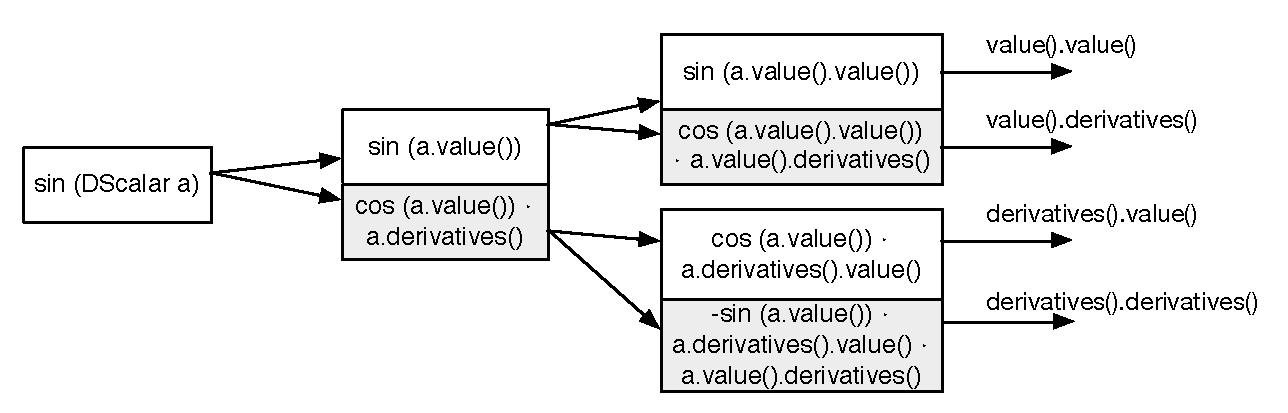
\includegraphics[width=\linewidth]{second-deriv}
\caption{C++ code generated by calling \texttt{sin} on a recursive AutoDiff (\texttt{DScalar}, defined in Section~\ref{section:second-derivs}). The middle box shows how templatizing the code in C++ generates \texttt{sin(AScalar)} and \texttt{cos(AScalar) * AScalar}, where \texttt{AScalar} is also defined in Section~\ref{section:second-derivs}.White boxes correspond to the \texttt{value()} ``field'', while gray boxes correspond to the \texttt{derivative} ``field'' returned at each level. \label{fig:second-derivs}}
\end{figure}

%\paragraph{What are the semantics of the various fields in the recursion?}

\subsection*{Semantics of the various fields in the recursion}

Where the first-derivative possessed clear semantices for \texttt{AScalar::derivatives()} on entry (i.e., it is equivalent to the output from the chain rule, as described in \S\ref{section:chain-rule}), the semantics of the fields for the recursive AutoDiff scalar are less meaningful.\\ \vspace{5mm}

\subsubsection*{For computing the second derivative of non-composite function $f(x)$, where $x$ is an independent variable}
We assume below that the AutoDiff scalar is named \texttt{a}. ``Input'' shows the proper settings for \texttt{a} on entry and ``Output'' shows the outputs on return from the C++ implementation of \texttt{f(a)}.
\begin{center}
\begin{tabular}{lll}
 & Input (\texttt{a}) & Output (\texttt{f(a)}) \\
\texttt{a.value().value()} & $x$ & $f(x)$ \\
\texttt{a.value().derivatives()} & $1$ & $\frac{df}{dx}(x)$ \\
\texttt{a.derivatives()(0).value()} & $1$ & $\frac{df}{dx}(x)$\\
\texttt{a.derivatives()(0).derivatives()} & --- & $\frac{d^2f}{dx^2}(x)$
\end{tabular}
\end{center}

\subsubsection*{For computing the second derivative of composite function $g(u)$ where $u = f(x)$ and $x$ is an independent variable}
We assume below that there are two AutoDiff scalars, named \texttt{a} and \texttt{b}. ``Input'' shows the proper settings for \texttt{a} and \texttt{b} on entry and ``Output'' shows the outputs on return from the C++ implementations of \texttt{f(a)} and \texttt{g(b)}.
\begin{center}
\begin{tabular}{lll}
 & Input (\texttt{a}) & Output (\texttt{f(a)}) \\
\texttt{a.value().value()} & $x$ & $f(x)$ \\
\texttt{a.value().derivatives()} & $1$ & $\frac{df}{dx}(x)$ \\
\texttt{a.derivatives()(0).value()} & $1$ & $\frac{df}{dx}(x)$\\
\texttt{a.derivatives()(0).derivatives()} & $0$ & $\frac{d^2f}{dx^2}(x)$
\end{tabular}
\end{center}
\textbf{Note that the zero input setting for \texttt{a.derivatives()(0).derivatives()} is not a misprint}. We now consider \texttt{b} and \texttt{f(b)}:
\begin{center}
\begin{tabular}{lll}
 & Input (\texttt{b}) & Output (\texttt{g(b)}) \\
\texttt{b.value().value()} & $u = f(x)$ & $g(u)$ \\
\texttt{b.value().derivatives()} & $\frac{du}{dx} = \frac{df}{dx}(x)$ & $\frac{dg}{du}\frac{du}{dx}(x)$ \\
\texttt{b.derivatives()(0).value()} & $\frac{du}{dx} = \frac{df}{dx}(x)$ & $\frac{dg}{du}\frac{du}{dx}(x)$\\
\texttt{b.derivatives()(0).derivatives()} & $\frac{d^2u}{dx^2}(x)$ & $\frac{d^2g}{dx^2}(x)$
\end{tabular}
\end{center}

The following code illustrates these concepts:
\begin{lstlisting}[language=C++]
#include <iostream>
#include <functional>
#include <Eigen/Core>
#include <unsupported/Eigen/AutoDiff>

// Typedef for a vector of two autodiff scalars (feature requires C++11). 
template <class T> using Vector1 = Eigen::Matrix<T, 1, 1>;

// Typedef for an AutoDiff scalar holding an scalar derivative.
typedef Eigen::AutoDiffScalar<Vector1<double>> AScalar;

// Typedef for a recursive AutoDiff scalar.
typedef Eigen::AutoDiffScalar<Vector1<AScalar>> DScalar;

template <class T>
T f(const T& x) {
  return x*x*x;
}

template <class T>
T g(const T& u) {
  return sin(u);
}

int main() {
  // Computes the second derivative of g(f(x)) evaluated at x = 4
  DScalar a;
  a.value() = 4;

  // Compute and output first and second derivatives from b = f(a)
  a.derivatives()(0).value() = 1;
  a.value().derivatives()(0) = 1;
  DScalar b = f(a);
  std::cout << "u = f(x) = x^3 = " << b.value().value() << " for x = " << a.value() << std::endl;
  std::cout << "du/dx = d/dx x^3 = 3*x^2 = " << b.derivatives()(0).value() << " = " << b.value().derivatives()(0) << " for x = " << a.value() << std::endl;
  std::cout << "d^2u/dx^2 = d^2/dx^2 x^3 = 6*x = " << b.derivatives()(0).derivatives() << " for x = " << a.value() << std::endl;
  
  // Compute and output first and second derivatives from g(b)
  std::cout << "g(u) = sin(u) = " << g(b).value().value() << " for u = " << b.value().value() << std::endl;
  std::cout << "dg/dx = cos(u) * du/dx (x) = " << g(b).value().derivatives()(0) << " = " << g(b).derivatives()(0).value() << " at x = " << a.value() << std::endl;
  std::cout << "d^2g/dx^2 = -sin(u) * (du/dx)^2 + cos(u) * d^2u/dx^2 (x) = " << g(b).derivatives()(0).derivatives()(0) << " at x = " << a.value() << std::endl;
}
\end{lstlisting}
The output of running this program is:
\begin{lstlisting}[language=bash]
u = f(x) = x^3 = 64 for x = 4
du/dx = d/dx x^3 = 3*x^2 = 48 = 48 for x = 4
d^2u/dx^2 = d^2/dx^2 x^3 = 6*x = 24 for x = 4
g(u) = sin(u) = 0.920026 for u = 64
dg/dx = cos(u) * du/dx (x) = 18.8091 = 18.8091 at x = 4
d^2g/dx^2 = -sin(u) * (du/dx)^2 + cos(u) * d^2u/dx^2 (x) = -2110.34 at x = 4
\end{lstlisting}
Please verify for yourself that these calculations match.

\bibliographystyle{abbrv}
%\bibliography{weazelball}

\end{document}
